% --------------------------------------------------
%  TALLER DE INTRODUCCIÓN A LaTeX
%  https://github.com/mianfg/latex-intro
%
%  Sesión 1 -> Presentación
%
%  Autor: Miguel Ángel Fernández Gutiérrez, @mianfg
%  Fecha: 20 febrero, 2019
% --------------------------------------------------

% Tipo de documento (presentación)
\documentclass[10pt, xcolor=table]{beamer}
\usepackage{caption}
\usepackage{subcaption}

% Cargar el tema
\usetheme{metropolis}

%  __________
% |          |
% | Paquetes |
% |__________|

% Paquetes de idioma
\usepackage[utf8]{inputenc}
\usepackage[spanish, es-tabla, es-lcroman, es-noquoting]{babel}

% Paquete para código fuente
% LISTINGS
\usepackage{listings}
\usepackage{lipsum}
\usepackage{courier}
\usepackage{csvsimple}

% Colores para los bloques de código
\definecolor{codegreen}{rgb}{0,0.6,0}
\definecolor{codegray}{rgb}{0.5,0.5,0.5}
\definecolor{codepurple}{rgb}{0.58,0,0.82}
\definecolor{backcolour}{rgb}{0.95,0.95,0.92}
\lstdefinestyle{mystyle}{
	backgroundcolor=\color{backcolour},   
	commentstyle=\color{codegreen},
	keywordstyle=\color{blue},
	numberstyle=\tiny\color{codegray},
	stringstyle=\color{codepurple},
	basicstyle=\footnotesize\ttfamily,
	breakatwhitespace=false,         
	breaklines=true,                 
	captionpos=b,                    
	keepspaces=true,                 
	numbers=left,                    
	numbersep=5pt,                  
	showspaces=false,                
	showstringspaces=false,
	showtabs=false,                  
	tabsize=4
}
\lstset{style=mystyle}

% Paquete de numeración en Beamer
\usepackage{appendixnumberbeamer}

% Paquete de uso para plantilla
\usepackage{booktabs}
\usepackage[scale=2]{ccicons}

% Paquete para controlar espacios
\usepackage{xspace}
\newcommand{\themename}{\textbf{\textsc{metropolis}}\xspace}

% Paquetes para matemáticas
\usepackage{amsmath}    % Paquete básico de matemáticas
\usepackage{amsthm}     % Teoremas
\usepackage{mathrsfs}   % Fuente para ciertas letras utilizadas en matemáticas

% Paquetes para fuentes
\usepackage{newpxtext, newpxmath}   % Fuente similar a Palatino
\usepackage{FiraSans}               % Fuente sans serif
\usepackage[T1]{fontenc}
\usepackage[italic]{mathastext}     % Utiliza la fuente del documento
                                    % en los entornos matemáticos

%  ________________________
% |                        |
% | Configuración del tema |
% |________________________|

% Configuración básica del tema
\metroset{
  % tema oscuro ('dark') o claro ('light'). No tiene efecto al usar la
  % paleta de colores más adelante
  background=light,
  % 'none' para eliminar la diapositiva inicial de cada sección
  sectionpage=progressbar,
  % 'progressbar' o 'simple' para añadir una diapositiva inicial a cada subsección
  subsectionpage=none,
  % contador de página: 'none', 'counter' o 'fraction'
  numbering=none,
  % barra de progreso: 'none', 'head', 'frametitle' o 'foot'
  progressbar=frametitle,
  % fondo de los bloques estilo teorema: 'transparent' o 'fill'
  block=fill,
}

% Paleta de colores
\definecolor{accent}{HTML}{009688}
\colorlet{darkaccent}{accent!70!black}
\definecolor{foreground}{RGB}{0, 0, 0}
\definecolor{background}{RGB}{255, 255, 255}

% Insertar los colores en el tema
\setbeamercolor{normal text}{fg=foreground, bg=background}
\setbeamercolor{alerted text}{fg=darkaccent, bg=background}
\setbeamercolor{example text}{fg=foreground, bg=background}
\setbeamercolor{frametitle}{fg=background, bg=accent}

\setbeamercolor{headtitle}{fg=background!70!accent,bg=accent!90!foreground}
\setbeamercolor{headnav}{fg=background,bg=accent!90!foreground}
\setbeamercolor{section in head/foot}{fg=background,bg=accent}

\defbeamertemplate*{headline}{miniframes theme no subsection}{
  % Caja para mostrar título y autor encima de cada diapositiva
  % Nosotros no 
  %% \begin{beamercolorbox}[ht=2.5ex,dp=1.125ex,
  %%     leftskip=.3cm,rightskip=.3cm plus1fil]{headtitle}
  %%   {\usebeamerfont{title in head/foot}\insertshorttitle}
  %%   \hfill
  %%   \leavevmode{\usebeamerfont{author in head/foot}\insertshortauthor}
  %% \end{beamercolorbox}
  %% \begin{beamercolorbox}[colsep=1.5pt]{upper separation line head}
  %% \end{beamercolorbox}

  % Caja para mostrar navegación encima de cada diapositiva
  \begin{beamercolorbox}{headnav}
    \vskip2pt\insertnavigation{\paperwidth}\vskip2pt
  \end{beamercolorbox}
  \begin{beamercolorbox}[colsep=1.5pt]{lower separation line head}
  \end{beamercolorbox}
}

%  _________
% |         |
% | Ajustes |
% |_________|

% Fijar tabla a posición
\usepackage{array}
\newcolumntype{L}[1]{>{\raggedright\let\newline\\\arraybackslash\hspace{0pt}}m{#1}}
\newcolumntype{C}[1]{>{\centering\let\newline\\\arraybackslash\hspace{0pt}}m{#1}}
\newcolumntype{R}[1]{>{\raggedleft\let\newline\\\arraybackslash\hspace{0pt}}m{#1}}

%  ________
% |        |
% | Título |
% |________|

\title{Divide y Vencerás}
\subtitle{Algorítmica. \alert{Práctica 2}}
\date{}
\author{Jose Alberto Hoces Castro\\Javier Gómez López\\Moya Martín Castaño\\[4pt]}
\titlegraphic{\hfill
\includegraphics[width=2.5cm]{logo_dark.jpg}}

%  ___________
% |           |
% | Documento |
% |___________|

\begin{document}
\maketitle

\begin{frame}{Contenidos}
	\setbeamertemplate{section in toc}[sections numbered]
	\tableofcontents[]
\end{frame}

\section{Introducción}
\begin{frame}[fragile]{Problemas planteados}
	\begin{itemize}
		\item \textbf{Ejercicio 1}: Buscar en un vector ordenado un elemento tal que \(v[i] = i\).
		\item \textbf{Ejercicio 2}: Dados \(k\) vectores ordenados, de \(n\) elementos cada uno, combinarlos en un vector ordenado.
	\end{itemize}
\end{frame}

\begin{frame}[fragile]{Objetivo de la prática}
Apreciar la utilidad de la técnica divide y vencerás (DyV) para resolver problemas de forma más eficiente que otras alternativas más sencillas o directas.
\end{frame}

\section{Ejercicio 1}
\begin{frame}[fragile]{Búsqueda secuencial}
Es la manera más obvia de buscar en un vector. Empezamos en el primer elemento y lo vamos recorriendo hasta encontrar el elemento deseado. En caso de no encontrarlo, devolvemos un valor que indique error (en nuestro caso -1).
\end{frame}

\begin{frame}[fragile]{Búsqueda secuencial. \normalfont{Código}}
\lstinputlisting[language=C++]{./Codes/secuencial.cpp}
\end{frame}

\begin{frame}[fragile]{Búsqueda secuencial. \normalfont{Eficiencia teórica}}
Observamos claramente que
\[
	T(n) \in \mathcal{O}(n)
\]
\end{frame}

\begin{frame}[fragile]{Búsqueda secuencial. \normalfont{Eficiencia empírica}}
	\begin{table}[h!]
		\centering
		\footnotesize
		\scalebox{0.7}{
			\begin{tabular}{|c|c|}
				\hline
				\multicolumn{2}{|c|}{\textsf{Búsqueda secuencial}}
				\\\hline
				\bfseries Elementos (n) & \bfseries Tiempo (s)
				\csvreader{./data/secuencial.csv}{}
				{\\\hline\csvcoli&\csvcolii}
				\\\hline
			\end{tabular}
		}
		\caption{Experiencia empírica de la búsqueda a fuerza bruta}
	\end{table}
\end{frame}

\begin{frame}[fragile]{Búsqueda secuencial. \normalfont{Eficiencia híbrida}}
\begin{figure}[h!]
	\centering
	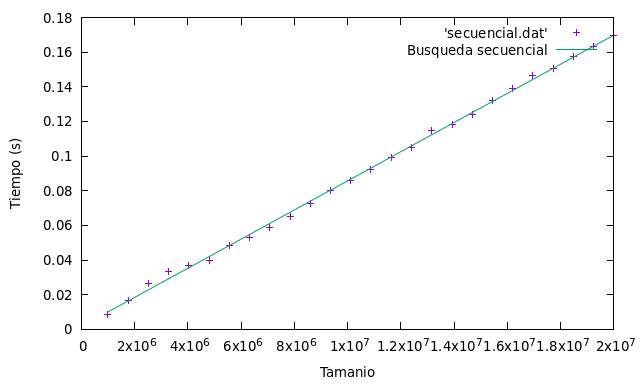
\includegraphics[scale=0.45]{./Images/Grafica_secuencial.png}
	\caption{Gráfica con los tiempos de ejecución de la búsqueda a fuerza bruta}
\end{figure}
\end{frame}

\begin{frame}[fragile]{Búsqueda binaria}
La tećnica Divide y Vencerás usada es la búsqueda binaria. Al estar ante un vector ordenado, podemos recurrir hasta algoritmo cuya eficiencia es logarítmica, mucho más preferible que una lineal.
\end{frame}

\begin{frame}[fragile]{Búsqueda binaria. \normalfont{Código}}
\lstinputlisting[language=C++]{./Codes/binaria.cpp}
\end{frame}

\begin{frame}[fragile]{Búsqueda binaria. \normalfont{Eficiencia teórica}}
Observamos claramente que 

\[
	T(n) = T\left(\frac{n}{2}\right) + a
\]
\centering $\downarrow$ 
\[
	(x-1)^2
\]
\centering $\downarrow$
\[
	T(2^k) = (c0+c1 \cdot k) \cdot 1^k
\]
\centering $\downarrow$
\[
	T(n) = c0 + c1 \cdot log(n)
\]
\centering $\downarrow$
\[
	T(n) \in \mathcal{O}(\log(n))
\]
\end{frame}

\begin{frame}[fragile]{Búsqueda binaria. \normalfont{Eficiencia empírica}}
 \begin{table}[h!]
	\centering
	\footnotesize
	\scalebox{0.7}{
		\begin{tabular}{|c|c|}
			\hline
			\multicolumn{2}{|c|}{\textsf{Búsqueda binaria}}
			\\\hline
			\bfseries Elementos (n) & \bfseries Tiempo (s)
			\csvreader{./data/binaria.csv}{}
			{\\\hline\csvcoli&\csvcolii}
			\\\hline
		\end{tabular}
	}
	\caption{Experiencia empírica de la búsqueda binaria}
\end{table}
\end{frame}


\begin{frame}[fragile]{Búsqueda binaria. \normalfont{Eficiencia híbrida}}
 \begin{figure}[h!]
	\centering
	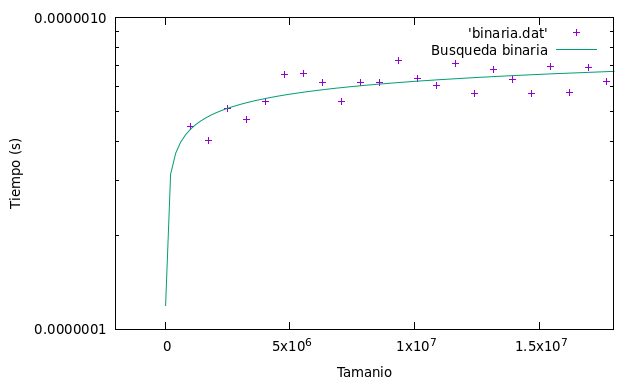
\includegraphics[scale=0.45]{./Images/Grafica_binaria.png}
	\caption{Gráfica con los tiempos de ejecución de la búsqueda binaria}
\end{figure}
\end{frame}

\begin{frame}[fragile]{Búsqueda binaria. \normalfont{Fuerza bruta vs Divide y Vencerás}}
	\begin{figure}[h!]
		\centering
		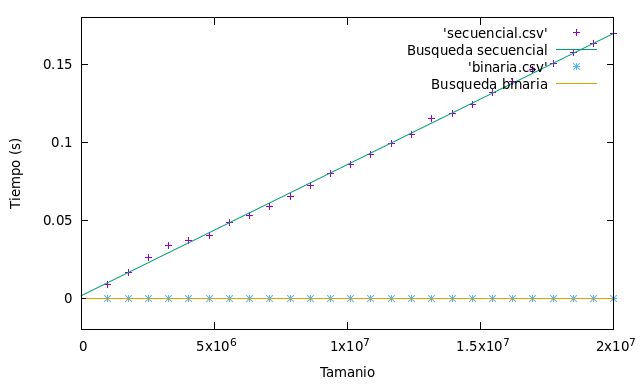
\includegraphics[scale=0.45]{./Images/Grafica_secvsbin.png}
		\caption{Gráfica comparativa: Fuerza Bruta vs DyV sin repeticiones}
	\end{figure}
\end{frame}

\begin{frame}[fragile]{Búsqueda binaria. \normalfont{Fuerza bruta vs Divide y Vencerás}}
Las expresiones del tiempo de cada algoritmo son:\\
\\
\centering Fuerza bruta $\longrightarrow$ \( T(n) = 8.41755 \cdot 10^{-9} n + 0.00153755\).\\
\centering DyV sin repeticiones $\longrightarrow$ \( T(n) = 5.63832 \cdot 10^{-8} \cdot \log_{2}(n) - 6.87177 \cdot 10^{-7}\).

E igualando las expresiones obtenemos que: \\
\centering $\downarrow$ \\
\centering \textbf{Umbral: $n = 1$}

\end{frame}

\begin{frame}[fragile]{¿Elementos repetidos?}
¿Qué pasaría si tuviésemos elementos repetidos? Por ejemplo:
\[
	1 \quad 2 \quad 3 \quad 4 \quad 4 \quad 5 \quad 6 \quad 7
\]
\end{frame}

\begin{frame}[fragile]{¿Elementos repetidos?. \normalfont{Solución}}
\lstinputlisting[language=C++]{./Codes/binaria_repes.cpp}
\end{frame}

\begin{frame}[fragile]{¿Elementos repetidos?. \normalfont{Eficiencia teórica}}
	
\[
T(n) = 2 \cdot T \left( \frac{n}{2} \right) + a
\]
\centering $\downarrow$
\[
(x-1)(x-2)
\]
\centering $\downarrow$
\[
T(2^k) = c0 + c1*2^k
\]
\centering $\downarrow$
\[
T(n) = c0 + c1*n
\]
\centering $\downarrow$
\[
T(n) \in \mathcal{O}(n)
\]

\end{frame}


\begin{frame}[fragile]{¿Elementos repetidos?. \normalfont{Eficiencia empírica}}
	\begin{table}[h!]
		\centering
		\footnotesize
		\scalebox{0.7}{
			\begin{tabular}{|c|c|}
				\hline
				\multicolumn{2}{|c|}{\textsf{Divide y Vencerás con repeticiones}}
				\\\hline
				\bfseries Elementos (n) & \bfseries Tiempo (s)
				\csvreader{./data/binaria_repes.csv}{}
				{\\\hline\csvcoli&\csvcolii}
				\\\hline
			\end{tabular}
		}
		\caption{Experiencia empírica de la búsqueda con repeticiones}
	\end{table}
\end{frame}

\begin{frame}[fragile]{¿Elementos repetidos?. \normalfont{Eficiencia híbrida}}
	\begin{figure}[h!]
		\centering
		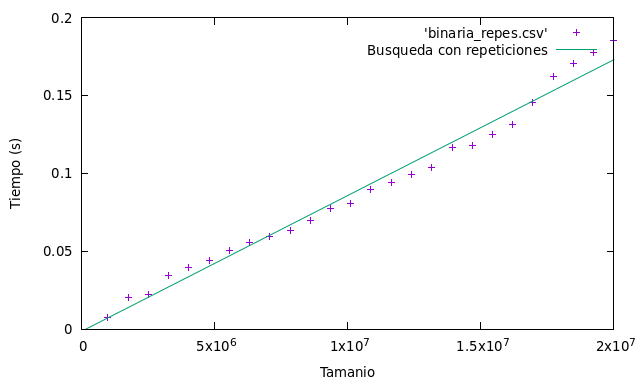
\includegraphics[scale=0.45]{./Images/Grafica_binaria_repes.png}
		\caption{Gráfica con los tiempos de ejecución de la búsqueda con repeticiones}
	\end{figure}
\end{frame}

\begin{frame}[fragile]{¿Elementos repetidos?. \normalfont{Fuerza bruta vs DyV con repeticiones}}
	\begin{figure}[h!]
		\centering
		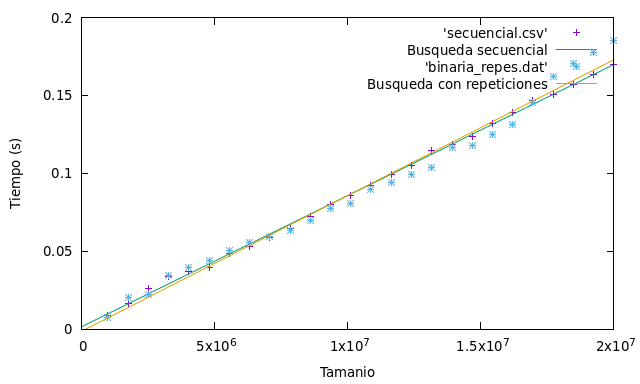
\includegraphics[scale=0.45]{./Images/Grafica_secvsrep.png}
		\caption{Gráfica comparativa: Fuerza Bruta vs DyV con repeticiones}
	\end{figure}
\end{frame}

\begin{frame}[fragile]{¿Elementos repetidos?. \normalfont{Fuerza bruta vs DyV con repeticiones}}
	\centering Fuerza bruta $\longrightarrow$ \( T(n) = 8.41755 \cdot 10^{-9} n + 0.00153755\).\\
	
	\centering DyV con repeticiones $\longrightarrow$ \( T(n) = 8.71886 \cdot 10^{-9} \cdot n -0.00140853 \).\\
	
	\centering $\downarrow$ \\
	
	\centering ¡La pendiente del algoritmo de fuerza bruta es menor que la del ``Divide y Vencerás''!
\end{frame}

\begin{frame}{Conclusiones}
	
	\item El uso de la técnica ``Divide y Vencerás'' no siempre es garantía de mejora respecto al uso del algoritmo de fuerza bruta.
	
	\item En aquellos casos en los que el uso de ``Divide y Vencerás'' sí nos ayuda a mejorar los tiempos, es importante saber que el algoritmo de fuerza bruta es preferible si se usan tamaños por debajo del umbral.
	
	\item EL uso de la recursividad requiere un uso excesivo de la pila y en algunos casos, esto da lugar a algoritmos ineficientes.
	
\end{frame}

\end{document}